\documentclass[]{article}

\usepackage[top=1in, bottom=1.25in, left=0.9in, right=0.9in]{geometry}
\usepackage{titlesec}
\titleformat{\section}
  {\normalfont\Large}
  {\thesection}{1em}{}
\titleformat{\subsection}
  {\normalfont\large}
  {\thesection}{1em}{}
\usepackage{wallpaper}
\ThisURCornerWallPaper{1.0}{img/cover.png}
\usepackage{color}
\usepackage{xcolor}
\usepackage{hyperref}
\definecolor{blue}{rgb}{0.01, 0.28, 1.0}
\definecolor{lightgray}{rgb}{0.95, 0.95, 0.95}
\hypersetup{colorlinks=true, urlcolor=blue, citecolor=blue, filecolor=blue, linkcolor=blue}
\makeatletter
\renewcommand{\maketitle}{\bgroup\setlength{\parindent}{0pt}
\begin{flushleft}
	\vspace{0.5cm}
 	\huge{\@title}\vspace{0.5cm}\\
	\quad\Large Homework (Session 5)\vspace{0.5cm}\\
  	\qquad\large\textit{\@author}
\end{flushleft}\egroup
}
\makeatother
\newcommand{\fakesection}[1]{
	\section*{#1}
	\par\refstepcounter{section}
	\addcontentsline{toc}{section}{#1}
}
\newcommand{\fakesubsection}[1]{
	\subsection*{#1}
	\par\refstepcounter{subsection}
	\addcontentsline{toc}{subsection}{\protect\numberline{\thesubsection}#1}
}
\newcommand{\fakesubsubsection}[1]{
	\subsubsection*{#1}
	\par\refstepcounter{subsubsection}
	\addcontentsline{toc}{subsubsection}{#1}
}
\newcommand{\parx}{\par\noindent}
\usepackage{tikz}
\usepackage{listings}
\usepackage{amssymb}

\usepackage[cachedir=minted]{minted}

%%%%%%%%%%%%%%%%%%%%%%%%%%%%%%%%%%%
%%%%%%%%%%%%%%%%%%%%%%%%%%%%%%%%%%%
%%%%%%%%%%%%%%%%%%%%%%%%%%%%%%%%%%%

\begin{document}

\title{Category Theory for Programmers}
\author{Bruno Vandekerkhove}
\date{}
\maketitle
\vspace{0.5cm}

\tableofcontents

\fakesection{Pushout in \texttt{C++}}

We talked about products and co-products in posets before, where the term supremum and infimum applied. In this more general case applied to \texttt{C++} types a diagram of a pushout $D$ is as follows :

\begin{center}
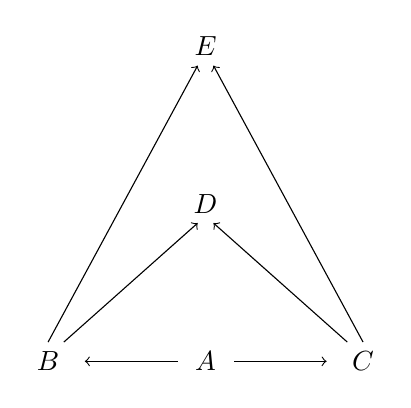
\begin{tikzpicture}
%\begin{scope}[yscale=1,xscale=-1]
	\node at (0,8) (1) {$E$};
	\node at (0,6) (4) {$D$};
	\node at (2,4) (2) {$C$};
	\node at (-2,4) (3) {$B$};
	\node at (0,4) (5) {$A$};
	\draw [<-] ([xshift=1mm]4.south) -- ([xshift=-2mm]2.north) node[midway,right] {$$};
	\draw [<-] ([xshift=-1mm]4.south) -- ([xshift=2mm]3.north) node[midway,left] {$$};
	\draw [<-] ([xshift=1mm]1.south) -- (2.north) node[midway,right] {$$};
	\draw [<-] ([xshift=-1mm]1.south) -- (3.north) node[midway,left] {$$};
	\draw [<-] ([xshift=2mm]3.east) -- ([xshift=-1mm]5.west) node[midway,right] {$$};
	\draw [<-] ([xshift=-2mm]2.west) -- ([xshift=1mm]5.east) node[midway,left] {$$};
%\end{scope}
\end{tikzpicture}
\end{center}

\noindent Any superclass $E$ of $B$ and $C$ is a superclass of $D$. Which means that $D$ corresponds to a superclass that encompasses all the functionality that the subclasses have in common\footnote{One has to consider all possible superclasses of $B$ and $C$. Then $D$ inherits from all of those. Some superclasses may only declare a part of the functionality that's present in both the classes $B$ and $C$, yet together they declare all of it and nothing more or some wouldn't be superclasses.}.

\fakesection{Limit of the identity functor}

The identity functor \texttt{Id} maps a category to itself. The initial object is the object for which there's exactly one morphism to every object. When constructing the limit for \texttt{Id} any apex will correspond to an initial object (or there wouldn't be a natural transformation from $\Delta_c$ to \texttt{Id}). If there are many apexes (or initial objects) there will be inversible transformations between them. Indeed, initial objects are unique up to isomorphism, which we knew already.

\fakesection{Pullback, pushout, ... in \texttt{Set}}

Starting from the diagram depicted on the previous page and applying analogous reasoning we can see that a pushout $D$ is the smallest superset or the union of $B$ and $C$. In the opposite category we get :

\begin{center}
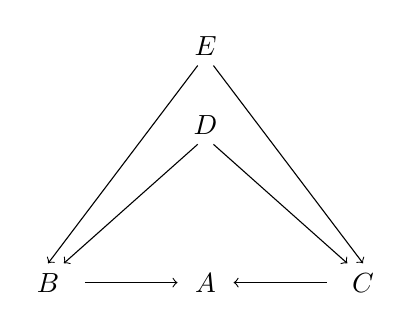
\begin{tikzpicture}
%\begin{scope}[yscale=1,xscale=-1]
	\node at (0,7) (1) {$E$};
	\node at (0,6) (4) {$D$};
	\node at (2,4) (2) {$C$};
	\node at (-2,4) (3) {$B$};
	\node at (0,4) (5) {$A$};
	\draw [->] ([xshift=1mm]4.south) -- ([xshift=-2mm]2.north) node[midway,right] {$$};
	\draw [->] ([xshift=-1mm]4.south) -- ([xshift=2mm]3.north) node[midway,left] {$$};
	\draw [->] ([xshift=1mm]1.south) -- (2.north) node[midway,right] {$$};
	\draw [->] ([xshift=-1mm]1.south) -- (3.north) node[midway,left] {$$};
	\draw [->] ([xshift=2mm]3.east) -- ([xshift=-1mm]5.west) node[midway,right] {$$};
	\draw [->] ([xshift=-2mm]2.west) -- ([xshift=1mm]5.east) node[midway,left] {$$};
%\end{scope}
\end{tikzpicture}
\end{center}

\noindent Here, the pullback $D$ is the largest subset or the intersection (every other set that's a subset of $B$ and $C$ ought to be a subset of $D$). A lattice visualises this and the terms supremum and infimum are in order.\\

\par\noindent As for the initial - and terminal object, they (trivially) correspond to the empty set and the set on which the category is based.

\fakesection{Co-equalizer}

Visually : 

\begin{center}
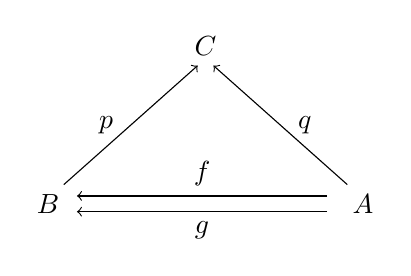
\begin{tikzpicture}
%\begin{scope}[yscale=1,xscale=-1]
	\node at (0,6) (4) {$C$};
	\node at (2,4) (2) {$A$};
	\node at (-2,4) (3) {$B$};
	\draw [<-] ([xshift=1mm]4.south) -- ([xshift=-2mm]2.north) node[midway,right,xshift=1mm] {$q$};
	\draw [<-] ([xshift=-1mm]4.south) -- ([xshift=2mm]3.north) node[midway,left,xshift=-1mm] {$p$};
	\draw [->] ([xshift=-2mm,yshift=1mm]2.west) -- ([xshift=1mm,yshift=1mm]3.east) node[midway,above,yshift=0mm] {$f$};
	\draw [->] ([xshift=-2mm,yshift=-1mm]2.west) -- ([xshift=1mm,yshift=-1mm]3.east) node[midway,below,yshift=0mm] {$g$};
%\end{scope}
\end{tikzpicture}
\end{center}

\noindent Once again $q$ is fully defined by $p$ and one of the morphisms from $A\rightarrow B$. We have 
$$q = p\cdot f\qquad and\qquad q = p\cdot g\qquad \Rightarrow\qquad p\cdot f = p\cdot g$$
where for every other co-equalizer $C'$ there should be a unique factoriser. Aside from this universal construction, there's a more concrete explanation of what it means in \texttt{Set}. There we end up with a partitioning of $B$ that corresponds to an equivalence relationship $f(x)\sim g(x)$. It should be the smallest of such relationships which corresponds to the finest partitioning\footnote{An example ; let $A=B=\{1,2,3\}$, $f=id$, $g(1)=2$, $g(2)=1$ and $g(3)=3$. Then we find a co-equalizer $p$ where $p(1)=p(2)=[1]$ and $p(3)=[3]$. This is a `\textit{better}' co-equalizer than $p'$ with $p'(x)=[1]$ because we find the factoriser $h$ with $h(x)=[1]$ for which $p'= h\cdot p$.}.
%.

\fakesection{Pullback towards terminal object, pushout from initial object}

A pullback is a special kind of product because $A$ imposes some additional structure. When you're dealing with $A$ as a terminal object and you're looking for a product, then that structure (morphisms to $A$ from $B$, $C$ and $D$) will necessarily be there. In other words, every such product is a pullback towards the terminal object (and vice versa, every such pullback is a product).\\

\par\noindent In the same vein, when you're dealing with $A$ as an initial object and are looking for a coproduct then there will be unique morphisms from $A$ to $B$, $C$ and $D$ which necessarily make it a pushout from the initial object.

%\bibliographystyle{plain}
%\bibliography{References}
%\addcontentsline{toc}{section}{References}

\end{document}